% Para facilitar a manutenção é sempre melhore criar um arquivo por capitulo, para exemplo isso não é necessário

%---------------------------------------------------------------------------------------
\chapter{Descrição da execução do experimento}

\section{Cenario 1}

	Foram necessários para o desenvolvimento do experimento:
	\begin{itemize}
		\item Multímetro Digital
		\item \ac{ci} de portas lógicas \textit{AND} ( \textit{datasheet} 7400 )
		\item \ac{ci} de portas lórigas \textit{OR}
		\item \ac{ci} de porta lógica inversora / \textit{NOT}( \textit{datashee} 7404)
		\item \textit{Protoboard}
		\item Fios para conectar as portas
		\item Fonte de Alimentação DC 5V
		\item LED Vermelho
		\item LED Verde
		\item 2 resistores para polarizar os LED’s
		\item Alicate
	\end{itemize}

	A partir do problema proposto, montou-se a seguinte expressão lógica
	$$ P . ( F + C + O) + (F . C . O)$$

	com P representando \textit{o voto do presidente}, F
	\textit{o voto do diretor financeiro}, C
	\textit{o voto do controller} e O \textit{o voto do diretor de operações}, após a
	montagem da expressão, foi elaborada a \autoref{table:tabelaVerdade1}. Com esta tabela e a expressão lógica,
	elaborou-se o circuito, conforme a \autoref{fig:desenhoCircuito1}. Com tais informações, foi repassado o circuito
	para o Quartus, depois renomeou-se as entradas e saídas para que, por meio do arquivo tradutor, a placa
	\ac{fpga} reconhecesse os componentes, conforme \autoref{fig:printCircuito1}.

	\begin{table}[h]
		\centering
		\caption{Tabela verdade da expressão lógica}\label{table:tabelaVerdade1}
		\begin{tabular}{c|c|c|c|c}
		%\hline
			\textbf{P} & \textbf{F} & \textbf{C} & \textbf{O} & \textbf{P.(F+C+O)+(F.C.O)} \\
			\hline
			0 & 0 & 0 & 0 & 0\\\hline
			0 & 0 & 0 & 1 & 0\\\hline
			0 & 0 & 1 & 0 & 0\\\hline
			0 & 0 & 1 & 1 & 0\\\hline
			0 & 1 & 0 & 0 & 0\\\hline
			0 & 1 & 0 & 1 & 0\\\hline
			0 & 1 & 1 & 0 & 0\\\hline
			0 & 1 & 1 & 1 & 1\\\hline
			1 & 0 & 0 & 0 & 1\\\hline
			1 & 0 & 0 & 1 & 1\\\hline
			1 & 0 & 1 & 0 & 1\\\hline
			1 & 0 & 1 & 1 & 1\\\hline
			1 & 1 & 0 & 0 & 1\\\hline
			1 & 1 & 0 & 1 & 1\\\hline
			1 & 1 & 1 & 0 & 1\\\hline
			1 & 1 & 1 & 1 & 1\\\hline

		\end{tabular}
	\end{table}

	\begin{figure}[H]
		\centering
		\caption{\label{fig:desenhoCircuito1}Desenho do circuito}
		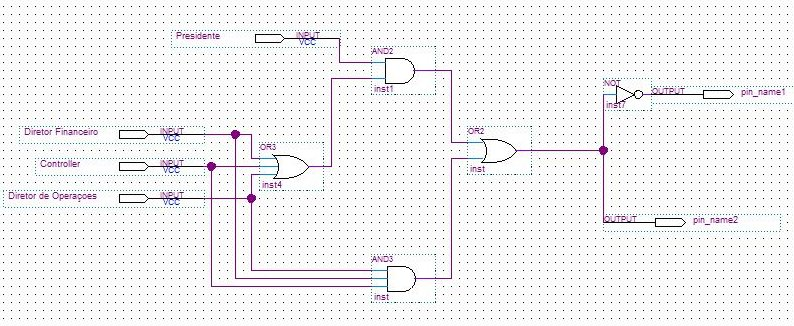
\includegraphics[width=1\textwidth]{img/cenario1/desenhoCircuito}
	\end{figure}

	\begin{figure}[H]
		\centering
		\caption{\label{fig:printCircuito1}Imagem do circuito no Quartus}
		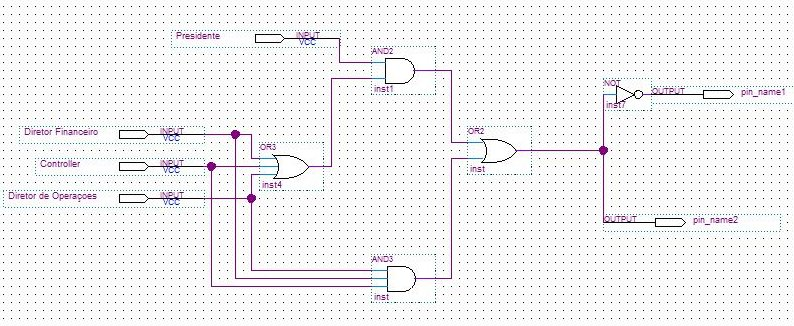
\includegraphics[width=1\textwidth]{img/cenario1/desenhoCircuito}
	\end{figure}

	\begin{figure}[H]
		\centering
		\caption{\label{fig:protoboard1}Configuração onde o LED Verde deveria acender (1001, por exemplo)}
		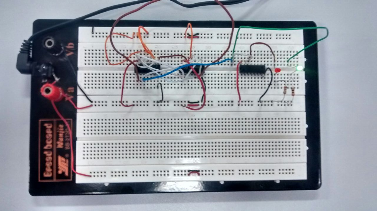
\includegraphics[width=1\textwidth]{img/cenario1/protoboard1}
	\end{figure}

	\begin{figure}[H]
		\centering
		\caption{\label{fig:protoboard2}Configuração onde o LED Vermelho deveria acender (0001, por exemplo)}
		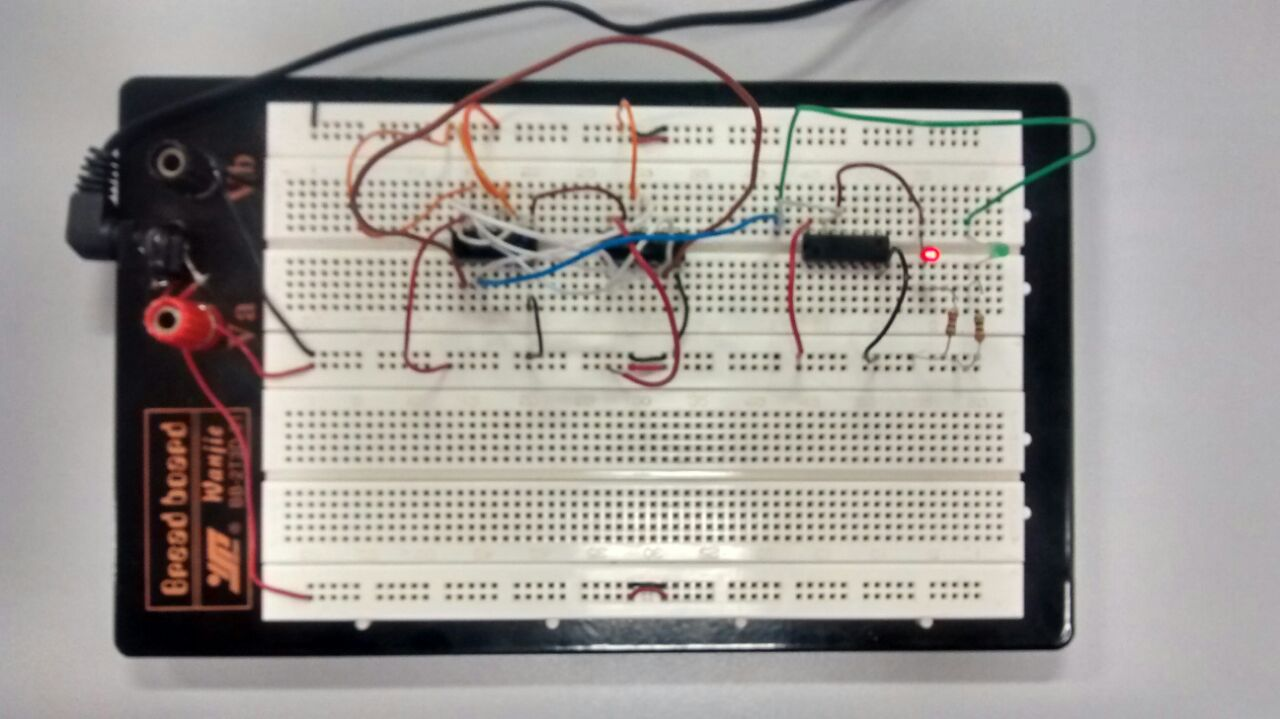
\includegraphics[width=1\textwidth]{img/cenario1/protoboard2}
	\end{figure}

\section{Cenario 2}
	Para a realização deste experimento, foram utilizados o programa Quartus 13.0 SP 1 e a placa \ac{fpga}
	Cyclone II - EP2C20F484C7.

	A partir do problema proposto, montou-se a seguinte expressão lógica
	$$ P + G + \sim V$$
	com P representando \textit{se a porta estiver aberta}, G
	\textit{se nível de gelo do congelador estiver acima do permitido} e V
	\textit{se o nível de gás do motor estiver adequado}, após a
	montagem da expressão, foi elaborada a \autoref{table:tabelaVerdade2}. Com esta tabela e a expressão lógica,
	elaborou-se o circuito, conforme a \autoref{fig:desenhoCircuito2}. Com tais informações, foi repassado o circuito
	para o Quartus, depois renomeou-se as entradas e saídas para que, por meio do arquivo tradutor, a placa
	\ac{fpga} reconhecesse os componentes.
	Para cobrir todos os casos de testes, foi realizada uma simulação, conforme a \autoref{fig:printSimulacao}.

	\begin{table}[h]
		\centering
		\caption{Tabela verdade da expressão lógica}\label{table:tabelaVerdade2}
		\begin{tabular}{c|c|c|c}
		%\hline
			\textbf{P} & \textbf{G} & \textbf{$\sim$V} & \textbf{P+G+($\sim$V)} \\
			\hline
			0 & 0 & 0 & 0\\\hline
			0 & 0 & 1 & 1\\\hline
			0 & 1 & 0 & 1\\\hline
			0 & 1 & 1 & 1\\\hline
			1 & 0 & 0 & 1\\\hline
			1 & 0 & 1 & 1\\\hline
			1 & 1 & 0 & 1\\\hline
			1 & 1 & 1 & 1
		\end{tabular}
	\end{table}

	\begin{figure}[H]
	    \centering
		\caption{\label{fig:desenhoCircuito2}Desenho do circuito}
		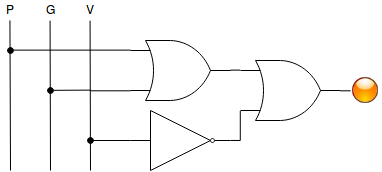
\includegraphics{img/cenario2/desenhoCircuito}
	\end{figure}


	\begin{figure}[H]
	    \centering
		\caption{\label{fig:printCircuito2}Imagem do circuinto no programa Quartus}
		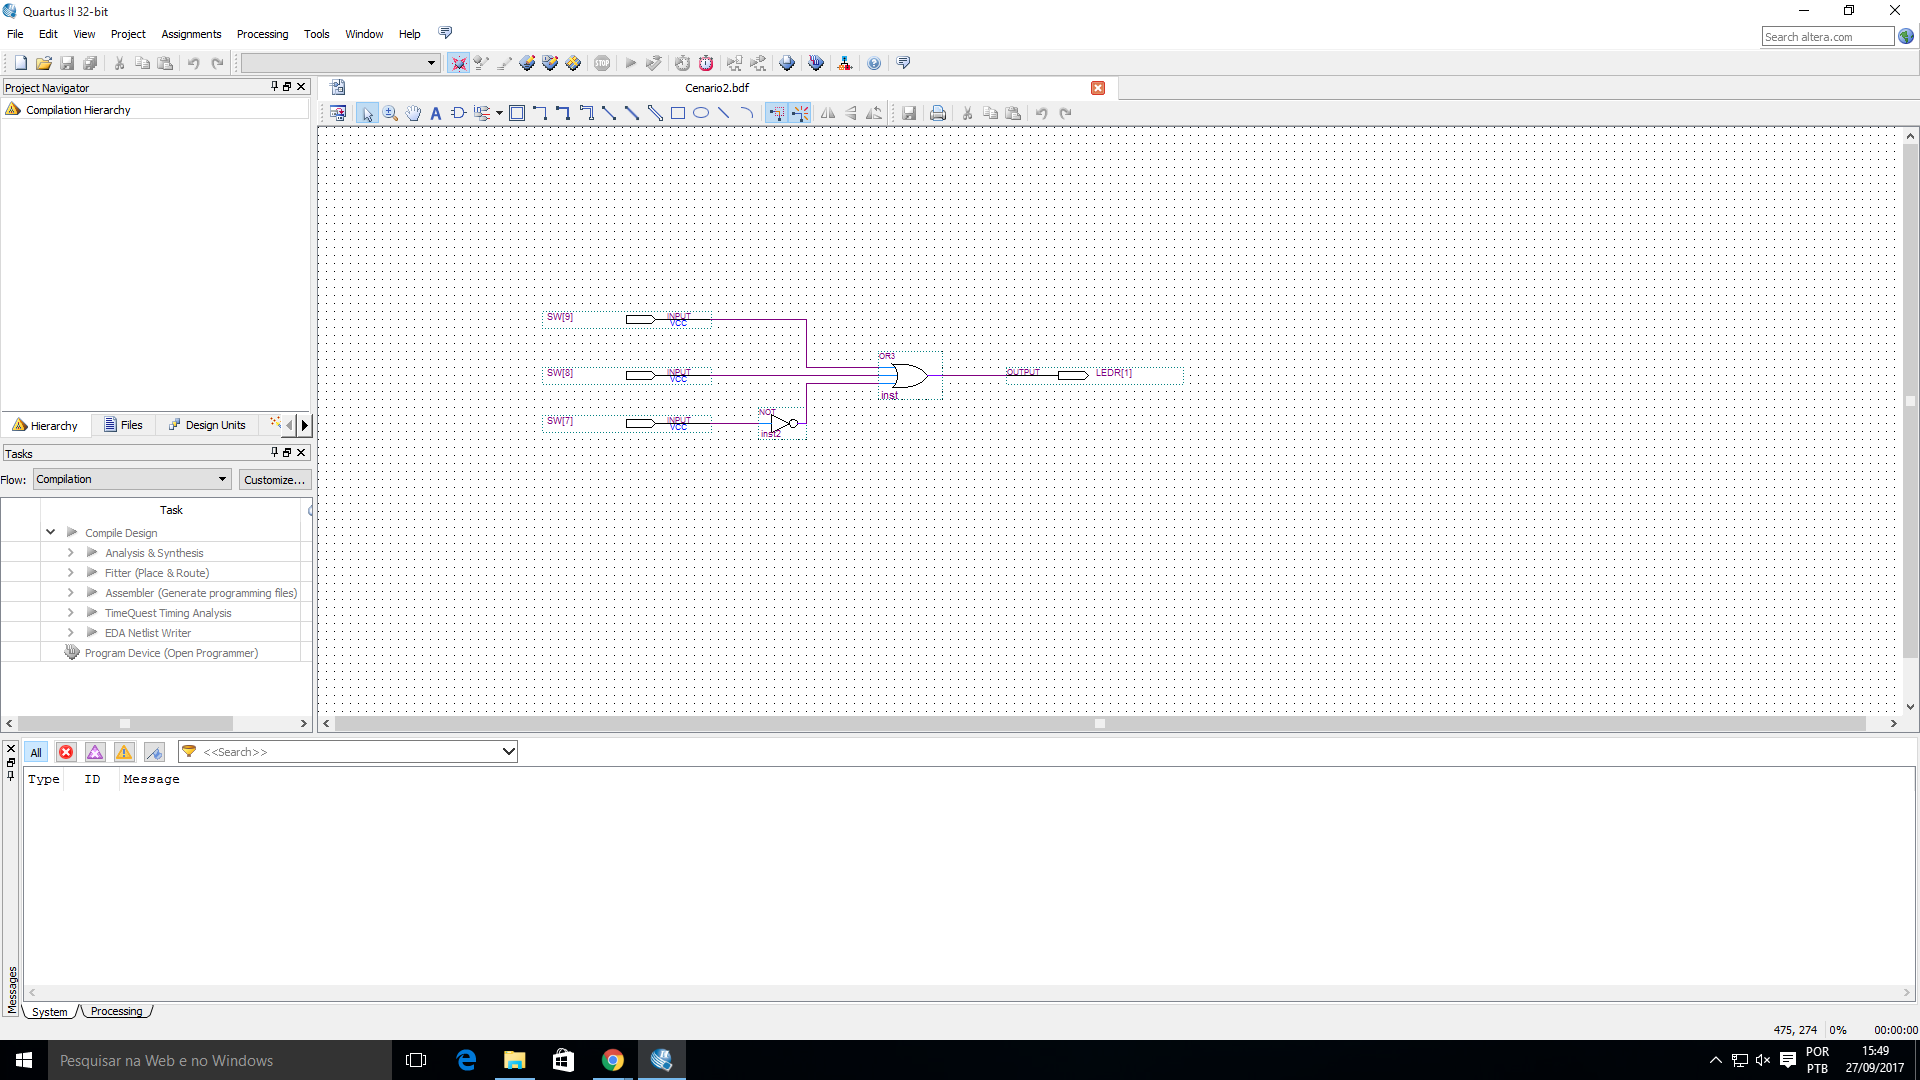
\includegraphics[width=1\textwidth]{img/cenario2/printCircuito}
	\end{figure}

	A porta SW[9] representa a P, a SW[8] representa a G, a SW[7]
	 representa a $\sim$V e a LEDR[1] é um led vermelho que irá
	 indicar o resultado provido da expressão lógica. Uma observação que não merece uma devida atenção é que
	 na \autoref{fig:desenhoCircuito2} foram necessárias a utilização de duas portas \textit{OR}, enquanto na
	 \autoref{fig:printCircuito2} foi necessária apenas a utilização de uma porta \textit{OR}. Isso ocorreu pelo fato
	 de que no Quartus existe a possibilidade de utilizar uma porta \textit{OR} de três entradas.

	Por fim, o circuito virtual foi compilado, conforme \autoref{fig:printCompilacao2}.

	\begin{figure}[H]
	    \centering
		\caption{\label{fig:printCompilacao2}Resultado da compilação do circuito}
		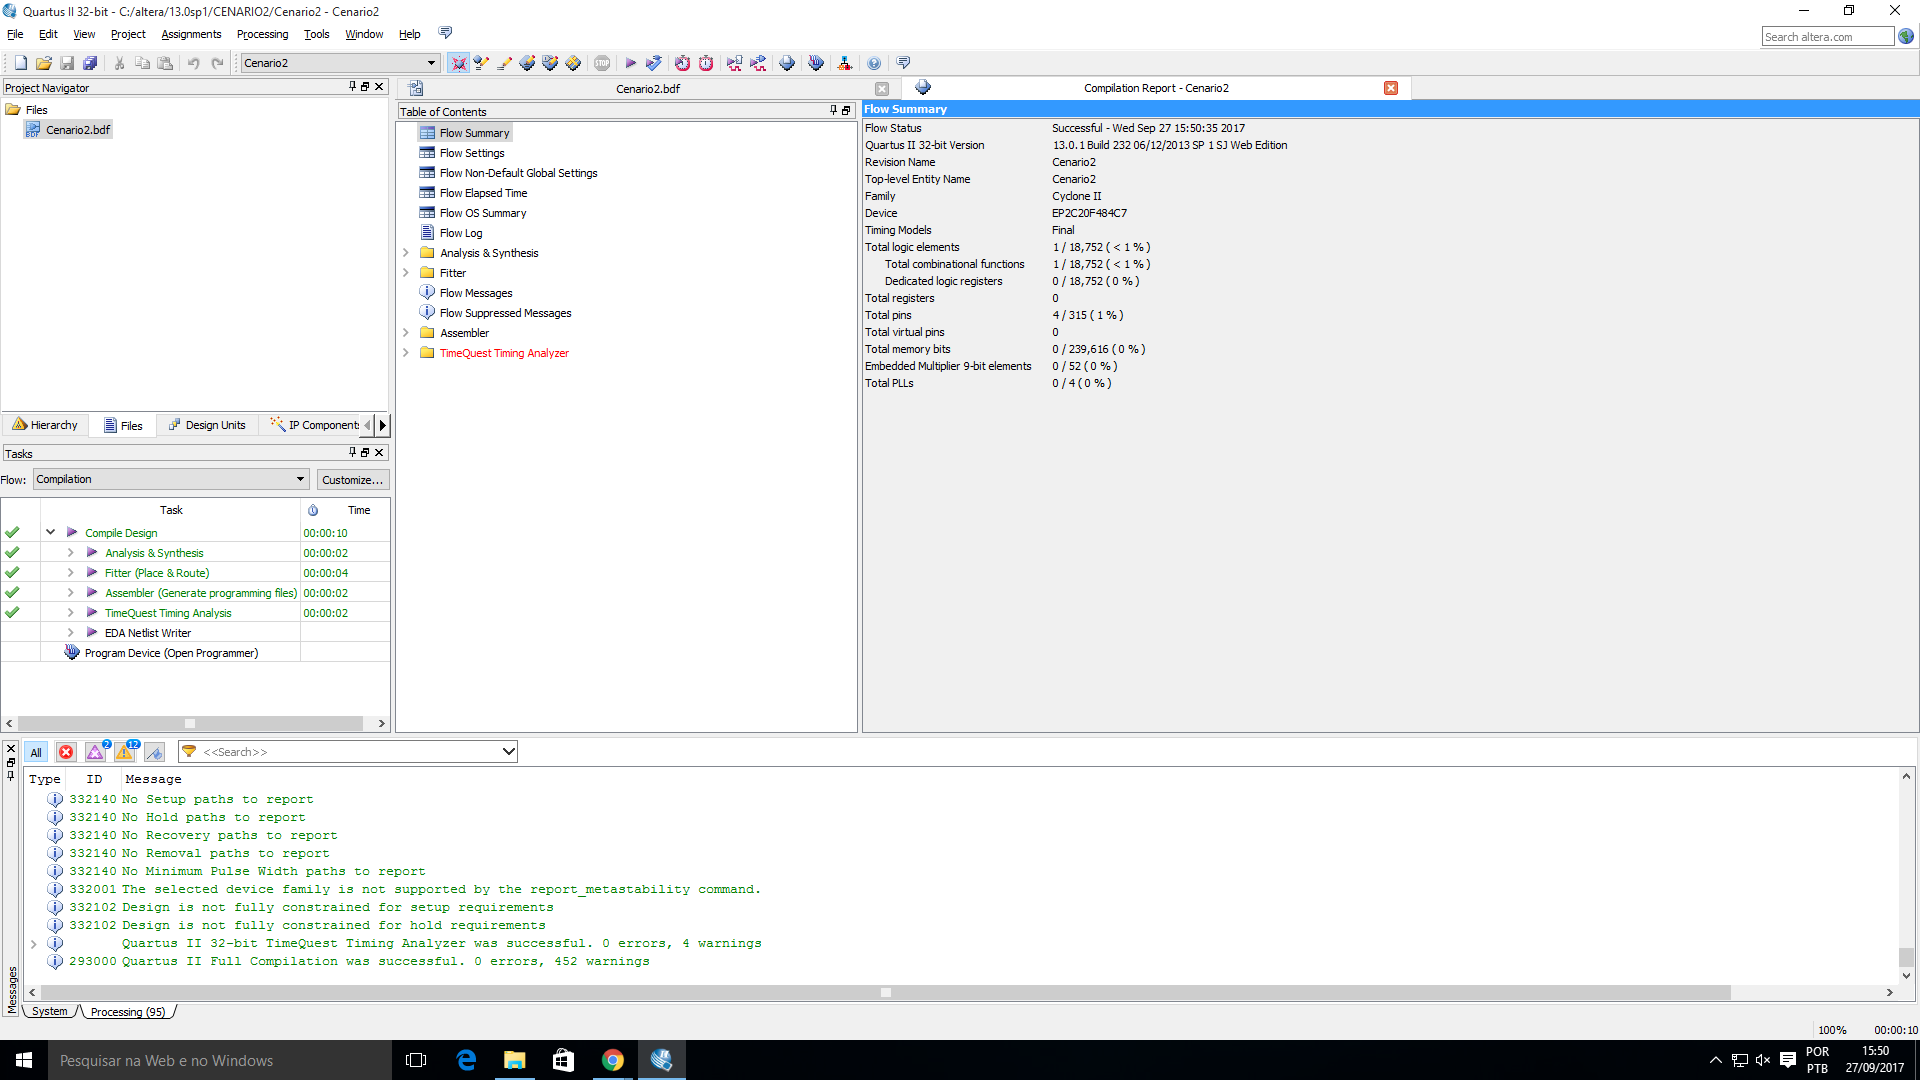
\includegraphics[width=1\textwidth]{img/cenario2/printCompilacao}
	\end{figure}


%Apresentar   o   detalhamento   da  execução  e   resultados   dos   passos   realizados
%durante   o   experimento,   incluindo   tabelas   verdade,   esquemáticos,   e   código
%(quando  houver).
%Especificar  componentes,  sistemas  e  instrumentos  utilizados.
%Usar listas, figuras e quadros, descrevê-los e discuti-los.
